\chapter{Ondas sonoras en los fluidos}\label{ch:b2:sound-waves}

Cuéntense los segundos entre el relámpago y el trueno y divídase por tres:
esa es la distancia en kilómetros. El sonido cruza el aire a un tercio de
kilómetro por segundo y el agua a kilómetro y medio, y un ecógrafo
cronometra los ecos que vienen del interior del cuerpo con una precisión
de una millonésima de segundo para dibujar su imagen. Este capítulo aplica
la mecánica de fluidos de \cref{ch:b2:euler-bernoulli,ch:b2:fluid-kinematics}
a un fluido en reposo perturbado por una pequeña ondulación de presión, y
vuelve a encontrar la \omterm{thm:b2:waves-on-strings:equation}{ecuación de d'Alembert}: la \omterm{thm:b2:sound-waves:equation}{velocidad del sonido}, qué
transporta la energía, cuánto es mucho ruido, cómo se propaga el sonido en
el espacio y por qué una sirena cambia de tono al pasar.

\section{La aproximación acústica}

\begin{definition}[Perturbación acústica]\label{def:b2:sound-waves:approximation}
\index{aproximación acústica}\index{sobrepresión}
Un fluido en reposo, de presión uniforme $P_0$ y densidad $\rho_0$, se
perturba: $P = P_0 + p(M, t)$, $\rho = \rho_0 + \rho_1(M, t)$, velocidad
$\vect v(M, t)$. La \emph{aproximación acústica} retiene solo el primer
orden en las magnitudes pequeñas $p$ (la \emph{sobrepresión}, o presión
acústica), $\rho_1$ y $\vect v$: $|p| \ll P_0$, $|\rho_1| \ll \rho_0$, $v \ll c$,
y la transformación que sufre cada \omterm{def:b2:fluid-kinematics:particle}{partícula de fluido} es tan rápida
que no intercambia calor: es \emph{isentrópica}, con la
compresibilidad $\chi_S = \frac1\rho\bigl(\frac{\partial\rho}{\partial P}\bigr)_S$.
Se desprecia la gravedad.
\end{definition}

\begin{theorem}[Ondas sonoras]\label{thm:b2:sound-waves:equation}
\index{velocidad del sonido}\index{ecuación de ondas (acústica)}
A primer orden, la \omterm{thm:b2:euler-bernoulli:euler}{ecuación de Euler}, la conservación de la masa y la ley
isentrópica se escriben
\[
\rho_0\frac{\partial\vect v}{\partial t} = -\operatorname{\vect{grad}}p , \qquad
\frac{\partial\rho_1}{\partial t} + \rho_0\operatorname{div}\vect v = 0 , \qquad
\rho_1 = \rho_0\chi_Sp ,
\]
y juntas dan la \omterm{thm:b2:waves-on-strings:equation}{ecuación de ondas} para la \omterm{def:b2:sound-waves:approximation}{sobrepresión},
\[
\Delta p = \frac1{c^2}\frac{\partial^2p}{\partial t^2} , \qquad
c = \frac1{\sqrt{\rho_0\chi_S}} ,
\]
(la misma para $\rho_1$ y para $\vect v$). Para un gas perfecto, $\chi_S =
1/\gamma P_0$ y
\[
c = \sqrt{\frac{\gamma P_0}{\rho_0}} = \sqrt{\frac{\gamma RT}{M}} :
\]
\qty{343}{m/s} en el aire a \qty{20}{\degreeCelsius}, con un aumento de
\qty{0.6}{m/s} por kelvin; \qty{1000}{m/s} en el helio; \qty{1480}{m/s} en el agua ($\chi_S =
\qty{4.5e-10}{Pa^{-1}}$).
\end{theorem}

\begin{proof}
Euler: el término convectivo $\rho(\vect v\cdot\operatorname{\vect{grad}})\vect v$
es de segundo orden, $\rho\,\partial_t\vect v \approx \rho_0\,\partial_t\vect v$, y
$\operatorname{\vect{grad}}P = \operatorname{\vect{grad}}p$. Masa: $\partial_t\rho +
\operatorname{div}(\rho\vect v) \approx \partial_t\rho_1 + \rho_0\operatorname{div}\vect v$.
Ley isentrópica: $\dd\rho = \rho\chi_S\,\dd P$ a primer orden. Tómese la
divergencia de la primera ecuación y la derivada temporal de la segunda:
$\rho_0\partial_t\operatorname{div}\vect v = -\Delta p = -\partial_t^2\rho_1 = -\rho_0\chi_S
\partial_t^2p$. Para el gas perfecto, $PV^\gamma$ constante a lo largo de una
transformación isentrópica da $\dd\rho/\rho = \dd P/\gamma P$, luego $\chi_S = 1/\gamma P$,
y $P_0/\rho_0 = RT/M$.
\end{proof}

\begin{remark}[Por qué isentrópica]\label{rem:b2:sound-waves:laplace}
Newton calculó la \omterm{thm:b2:sound-waves:equation}{velocidad del sonido} con la compresibilidad isoterma,
$\sqrt{P_0/\rho_0} = \qty{290}{m/s}$, un $15\%$ demasiado baja; Laplace vio
que las compresiones son demasiado rápidas para que el calor pase de las
crestas calientes a los valles fríos --- en un periodo el calor difunde
unos micrómetros (\cref{ch:b2:heat-conduction}), nada frente a una
longitud de onda ---, de modo que la transformación es adiabática y
reversible y aparece $\gamma$. La \omterm{thm:b2:sound-waves:equation}{velocidad del sonido} es así una medida
directa de $\gamma$: $1.40$ para el aire, $1.67$ para el argón.
\end{remark}

\begin{omfigure}
\begin{tikzpicture}[font=\small, x=1cm, y=1cm, >=Stealth]
  \begin{scope}
    \draw[thick] (-3.2,-0.8) rectangle (3.2,0.8);
    \fill[omDef!25] (-0.6,-0.8) rectangle (0.6,0.8);
    \fill[omDef!8] (-0.35,-0.8) rectangle (0.95,0.8);
    \draw[omDef, dashed] (-0.35,-0.8) -- (-0.35,0.8) (0.95,-0.8) -- (0.95,0.8);
    \draw[omThm, very thick, ->] (-1.6,0) -- (-0.65,0) node[above, font=\footnotesize, pos=0.3] {$P(x)S$};
    \draw[omThm, very thick, ->] (1.6,0) -- (0.65,0) node[above, font=\footnotesize, pos=0.3] {$P(x+\dd x)S$};
    \node[font=\footnotesize] at (-0.6,-1.1) {$x$}; \node[font=\footnotesize] at (0.65,-1.1) {$x + \dd x$};
    \draw[omDef, ->] (-0.6,1.05) -- (-0.35,1.05) node[above, font=\footnotesize, pos=1.4] {$\xi(x)$};
    \node[font=\footnotesize] at (0,-1.7) {$\rho_0\,\partial_t v = -\partial_x p$, \quad $\rho_1 = -\rho_0\,\partial_x\xi = \rho_0\chi_S\,p$};
  \end{scope}
  \begin{scope}[xshift=8.2cm]
    \foreach \x in {-2.6,-2.45,...,2.6} {
      \pgfmathsetmacro{\d}{0.18*sin(deg(2.4*\x))}
      \draw[omDef, thick] ({\x+\d},-0.8) -- ({\x+\d},0.8);
    }
    \node[font=\scriptsize] at (-1.6,-1.1) {compresión}; \node[font=\scriptsize] at (0,-1.1) {dilatación}; \node[font=\scriptsize] at (1.6,-1.1) {compresión};
    \draw[omThm, thick, ->] (-0.4,1.1) -- (0.8,1.1) node[right, font=\footnotesize] {$c$};
    \node[font=\footnotesize] at (0,-1.7) {una onda sonora plana: las láminas de fluido se apiñan y se separan};
  \end{scope}
\end{tikzpicture}

{\small A la izquierda, una lámina de fluido desplazada en $\xi(x, t)$ y
empujada por las presiones sobre sus caras; su compresión fija la
\omterm{def:b2:sound-waves:approximation}{sobrepresión}. A la derecha, una onda sonora plana: zonas alternas de
compresión y de dilatación que se mueven a $c$, con el propio fluido
oscilando adelante y atrás en la dirección de propagación (una \omterm{prop:b2:waves-on-strings:chain}{onda longitudinal}).}
\end{omfigure}

\section{Ondas planas, impedancia, intensidad}

\begin{proposition}[Onda sonora plana progresiva]\label{prop:b2:sound-waves:plane}
\index{impedancia acústica}\index{intensidad acústica}\index{densidad de energía (acústica)}
Para una onda plana $p = f(x - ct)$ que viaja hacia $+x$, la velocidad del
fluido va según $x$, en fase con la \omterm{def:b2:sound-waves:approximation}{sobrepresión}, y
\[
p = Z\,v , \qquad Z = \rho_0c = \sqrt{\rho_0/\chi_S} ,
\]
donde $Z$ es la \emph{\omterm{prop:b2:sound-waves:plane}{impedancia acústica}} del medio
(\unit{kg.m^{-2}.s^{-1}}): \qty{410}{kg.m^{-2}.s^{-1}} para el aire, \qty{1.5e6}{kg.m^{-2}.s^{-1}}
para el agua, $\sim\qty{1.6e6}{kg.m^{-2}.s^{-1}}$ para los tejidos blandos y
\qty{4e7}{kg.m^{-2}.s^{-1}} para el acero. La onda transporta la densidad de
energía y la intensidad (potencia por unidad de área, hacia $+x$)
\[
e = \tfrac12\rho_0v^2 + \tfrac12\chi_Sp^2 , \qquad I = p\,v ,
\]
que obedecen $\partial_te + \partial_xI = 0$; para la onda progresiva las dos
mitades de $e$ son iguales y $I = p^2/Z = Zv^2$. Una onda sinusoidal de
amplitud de presión $p_m$ tiene la intensidad media $\langle I\rangle = p_m^2/2Z$.
\end{proposition}

\begin{proof}
Para $p = f(x - ct)$, $\rho_0\partial_tv = -\partial_xp = f'/c\cdot c\dots$: con precisión,
$\rho_0\partial_tv = -f'(x - ct)$, y $v = f(x - ct)/\rho_0c$ lo cumple. El
término potencial de $e$ es el trabajo almacenado al comprimir el fluido
(una compresión isentrópica de un volumen unidad en $\dd V/V = -\chi_S\,\dd p$
almacena $\int p\,\chi_S\dd p = \tfrac12\chi_Sp^2$); $I$ es la potencia de la
fuerza de presión $pS$ sobre el fluido de delante, que se mueve a $v$, por unidad de área.
Balance: $\partial_te = \rho_0v\partial_tv + \chi_Sp\partial_tp = -v\partial_xp - p\partial_xv =
-\partial_x(pv)$ en virtud de las dos ecuaciones linealizadas.
\end{proof}

\begin{definition}[Nivel sonoro]\label{def:b2:sound-waves:decibel}
\index{decibelio}\index{nivel sonoro}\index{umbral de audición}
El \emph{nivel sonoro} de una onda de intensidad media $I$ vale
\[
L = 10\log_{10}\frac I{I_0} \ \text{dB} , \qquad I_0 = \qty{1e-12}{W/m^2}
\]
--- el umbral de audición a \qty{1}{kHz}, que corresponde en el aire a la
amplitud de presión $p_0 \approx \qty{2e-5}{Pa}$ (eficaz) $= 2 \times 10^{-10}$
atmósferas. Duplicar la intensidad añade \qty{3}{dB}; multiplicarla por diez, \qty{10}{dB};
multiplicar por cien la amplitud de presión, \qty{40}{dB}. Habitación silenciosa
\qty{30}{dB}, conversación \qty{60}{dB}, calle con tráfico \qty{80}{dB}, concierto de rock
\qty{110}{dB}, dolor \qty{120}{dB} ($I = \qty{1}{W/m^2}$, $p_m = \qty{29}{Pa}$).
\end{definition}

\begin{example}[Qué pequeño es un sonido]\label{ex:b2:sound-waves:small}
En el umbral, a \qty{1}{kHz}: $p_m = \qty{2.8e-5}{Pa}$, $v_m = p_m/Z =
\qty{7e-8}{m/s}$, y la amplitud de desplazamiento $\xi_m = v_m/\omega =
\qty{1e-11}{m}$ --- una décima de diámetro atómico: el tímpano detecta
movimientos menores que un átomo. A \qty{120}{dB}, $\xi_m = \qty{11}{\micro m}$,
todavía invisible, y $p_m/P_0 = 3 \times 10^{-4}$: incluso los sonidos más
fuertes son perturbaciones minúsculas, y por eso funciona tan bien la teoría lineal.
\end{example}

\begin{omfigure}
\begin{tikzpicture}
\begin{axis}[omaxis, axis x line=middle, axis y line=left, width=7.4cm, height=4.2cm,
    xlabel={$x$}, ylabel={}, xmin=0, xmax=6.6, ymin=-1.3, ymax=1.4, xtick=\empty, ytick=\empty, samples=100,
    xlabel style={at={(axis description cs:1.0,0.5)}, anchor=west},
    legend style={font=\scriptsize, at={(0.5,1.02)}, anchor=south, legend columns=3, draw=none, fill=none}]
  \addplot[omThm, thick, domain=0:6.28] {sin(deg(x))};
  \addplot[omDef, thick, dashed, domain=0:6.28] {sin(deg(x))};
  \addplot[omProp, thick, domain=0:6.28] {cos(deg(x))};
  \legend{$p$, $v = p/Z$, $\xi$}
\end{axis}
\end{tikzpicture}
\hfill
\begin{tikzpicture}[font=\small, x=1cm, y=1cm, >=Stealth]
  \draw[thick, ->] (0,0) -- (0,4.4);
  \foreach \l/\t in {0/umbral de audición, 1/hojas al viento, 2/habitación silenciosa, 3/conversación, 4/calle con tráfico, 5/camión a \qty{10}{m}, 6/concierto de rock, 7/dolor} {
    \pgfmathsetmacro{\y}{0.6*\l}
    \draw (-0.1,\y) -- (0.1,\y);
    \node[anchor=east, font=\scriptsize] at (-0.15,\y) {\pgfmathparse{int(20*\l)}\pgfmathresult~dB};
    \node[anchor=west, font=\scriptsize] at (0.15,\y) {\t};
  }
  \node[font=\scriptsize, anchor=south] at (0,4.45) {$I$ ($\times 100$ por escalón)};
\end{tikzpicture}

{\small A la izquierda, en una onda sonora plana progresiva la
\omterm{def:b2:sound-waves:approximation}{sobrepresión} y la velocidad del fluido están en fase, y el desplazamiento
se retrasa un cuarto de periodo. A la derecha, la escala de \omterm{def:b2:sound-waves:decibel}{decibelios}:
cada escalón de \qty{20}{dB} multiplica la intensidad por cien y la amplitud de presión por diez.}
\end{omfigure}

\section{Ondas esféricas}

\begin{proposition}[Ondas esféricas y la ley del inverso del cuadrado]\label{prop:b2:sound-waves:spherical}
\index{onda esférica}\index{ley del inverso del cuadrado (sonido)}
Una fuente pequeña que radia por igual en todas las direcciones produce la
\omterm{prop:b2:sound-waves:spherical}{onda esférica}
\[
p(r, t) = \frac{A}{r}\,f\Bigl(t - \frac rc\Bigr) ,
\]
cuya amplitud decrece como $1/r$ y cuya intensidad decrece como $1/r^2$:
para una fuente de potencia acústica $\mathcal P$, $I = \mathcal P/4\pi r^2$, es decir,
$-\qty{6}{dB}$ cada vez que se duplica la distancia. Lejos de la fuente la
onda es localmente plana, con $v = p/Z$ radial.
\end{proposition}

\begin{proof}
En coordenadas esféricas, para una función solo de $r$, $\Delta p =
\frac1r\frac{\partial^2(rp)}{\partial r^2}$ (admitido; \cref{ch:b2:maxwell-equations}),
de modo que $u = rp$ obedece la \omterm{thm:b2:waves-on-strings:equation}{ecuación de ondas} unidimensional $\partial_r^2u = \partial_t^2u/c^2$,
de donde $u = Af(t - r/c)$ para la onda saliente. La potencia que atraviesa una
esfera de radio $r$ vale $4\pi r^2I$, constante si nada se absorbe.
\end{proof}

\begin{example}[Una sirena, una conversación]\label{ex:b2:sound-waves:siren}
Una sirena de \qty{10}{W}: $I = 10/4\pi r^2$, \qty{0.8}{W/m^2} a \qty{1}{m} (\qty{119}{dB},
umbral de dolor), \qty{79}{dB} a \qty{100}{m}, \qty{59}{dB} a \qty{1}{km} --- todavía audible sobre
la ciudad. Una voz radia unos \qty{10}{\micro W}: \qty{60}{dB} a \qty{1}{m}
y \qty{40}{dB} a \qty{10}{m}. El aire también absorbe sonido (más a alta
frecuencia, unos \omterm{def:b2:sound-waves:decibel}{decibelios} por cada cien metros a \qty{10}{kHz}), y por eso
el trueno lejano retumba grave.
\end{example}

\section{El efecto Doppler}

\begin{theorem}[Efecto Doppler]\label{thm:b2:sound-waves:doppler}
\index{efecto Doppler}
Una fuente emite a la frecuencia $f$ y se mueve a la celeridad $v_s$ a lo
largo de la recta que la une con un observador que se mueve a $v_o$, con
ambas celeridades contadas positivas cuando se acercan; el sonido viaja a
$c$ en el aire en reposo. El observador recibe la frecuencia
\[
f' = f\,\frac{c + v_o}{c - v_s} .
\]
Una fuente en movimiento apiña sus frentes de onda por delante ($\lambda' = (c - v_s)/f$)
y los separa por detrás; un observador en movimiento encuentra frentes a
razón de $(c + v_o)/\lambda$. Para $v_s, v_o \ll c$ ambos dan $\Delta f/f \approx
(v_s + v_o)/c$.
\end{theorem}

\begin{proof}
Fuente en movimiento: los frentes emitidos en $t$ y en $t + 1/f$ están
separados por $c/f - v_s/f$ en la dirección del movimiento, de modo que la
longitud de onda por delante vale $\lambda' = (c - v_s)/f$ y la frecuencia
que recibe un observador fijo es $c/\lambda'$. Observador en movimiento: la
longitud de onda es $\lambda = c/f$, pero los frentes pasan a la celeridad
relativa $c + v_o$. Combínense.
\end{proof}

\begin{omfigure}
\begin{tikzpicture}[font=\small, x=1cm, y=1cm, >=Stealth]
  \begin{scope}
    \foreach \i in {0,1,2,3,4} {
      \pgfmathsetmacro{\r}{0.45*(5-\i)}
      \pgfmathsetmacro{\cx}{0.27*\i-0.23}
      \draw[omDef, thick] (\cx,0) circle (\r);
    }
    \fill[omThm] (1.12,0) circle (2pt);
    \draw[omThm, thick, ->] (1.12,0.15) -- (1.9,0.15) node[above, font=\footnotesize] {$v_s$};
    \node[font=\footnotesize] at (2.0,-2.45) {por delante: $\lambda' < \lambda$};
    \node[font=\footnotesize] at (-1.5,-2.45) {por detrás: $\lambda' > \lambda$};
    \node[font=\footnotesize] at (0.4,-3.2) {$f' = f\,\dfrac{c + v_o}{c - v_s}$};
  \end{scope}
  \begin{scope}[xshift=8.2cm]
    \foreach \i in {0,1,2,3,4} {
      \pgfmathsetmacro{\r}{0.4*(5-\i)}
      \pgfmathsetmacro{\cx}{0.6*\i-1.12}
      \draw[omDef, thick] (\cx,0) circle (\r);
    }
    \fill[omThm] (1.88,0) circle (2pt);
    \draw[omThm, thick, ->] (1.88,0.15) -- (2.7,0.15) node[above, font=\footnotesize] {$v > c$};
    \draw[omProp, thick] (1.88,0) -- (-0.36,2.0); \draw[omProp, thick] (1.88,0) -- (-0.36,-2.0);
    \draw (0.9,0) arc[start angle=180, end angle=138, radius=0.98] node[left, font=\footnotesize, xshift=-1pt] {$\theta$};
    \node[font=\footnotesize] at (0.3,-3.2) {cono de Mach: $\sin\theta = c/v$};
  \end{scope}
\end{tikzpicture}

{\small A la izquierda, los frentes de onda de una fuente en movimiento se
apiñan por delante y se separan por detrás: sonido más agudo al acercarse,
más grave al alejarse. A la derecha, una fuente más rápida que el sonido
deja atrás sus frentes de onda; su envolvente es el \omterm{rem:b2:sound-waves:mach}{cono de Mach}, que se
oye en el suelo como un estampido.}
\end{omfigure}

\begin{example}[Sirenas, cinemómetros, glóbulos rojos]\label{ex:b2:sound-waves:dopplerex}
La sirena de una ambulancia de \qty{700}{Hz} que pasa a \qty{25}{m/s}: \qty{755}{Hz}
al acercarse y \qty{651}{Hz} al alejarse --- una caída de un sexto de
octava, la conocida inflexión del ``nino-nino''. Un cinemómetro de la
policía mide el mismo efecto sobre una onda de radio de \qty{24}{GHz}
reflejada por un coche (la onda se desplaza dos veces, al recibirla el
coche y al reemitirla): $\Delta f = 2fv/c =
\qty{4.8}{kHz}$ a \qty{30}{m/s}. Una sonda de ultrasonidos de \qty{5}{MHz} apuntada a
una arteria oye los glóbulos a $\Delta f = 2fv\cos\theta/c \approx \qty{1.6}{kHz}$
para \qty{0.5}{m/s} a \qty{60}{\degree}: un silbido audible cuyo tono es la
celeridad de la sangre. Y las rayas espectrales de una galaxia que se aleja
se desplazan al rojo en $\Delta\lambda/\lambda = v/c$ --- la fórmula vale para la luz a baja velocidad,
con la corrección relativista más allá.
\end{example}

\begin{remark}[Supersónico]\label{rem:b2:sound-waves:mach}
\index{cono de Mach}\index{estampido sónico}
Cuando $v_s > c$ la fórmula deja de valer ($f' < 0$ por delante): ningún
sonido precede a la fuente. Los frentes de onda emitidos a lo largo de la
trayectoria tienen una envolvente cónica de semiángulo $\theta$ con $\sin\theta = c/v_s$ (el \emph{\omterm{rem:b2:sound-waves:mach}{cono de Mach}});
el salto de presión que lleva el cono es el \omterm{rem:b2:sound-waves:mach}{estampido sónico}, que llega a
un oyente del suelo solo después de que el avión haya pasado --- a
Mach $2$ y \qty{10}{km} de altitud, $\theta = \qty{30}{\degree}$ y el estampido
llega $10\,\text{km}/\tan\theta/v_s \approx \qty{25}{s}$ después del paso por
la vertical. El chasquido de una bala y la punta de un látigo son el mismo cono.
\end{remark}

\begin{method}[Órdenes de magnitud en acústica]\label{met:b2:sound-waves:method}
Dado un \omterm{def:b2:sound-waves:decibel}{nivel sonoro} $L$: $I = I_0\,10^{L/10}$; luego $p_m = \sqrt{2ZI}$,
$v_m = p_m/Z$, $\xi_m = v_m/\omega$; la potencia de una fuente vale $4\pi r^2I$ si
radia en todas las direcciones (la mitad sobre un suelo duro, que refleja
hacia un semiespacio). Pasar de $r_1$ a $r_2$ cambia $L$ en
$20\log_{10}(r_1/r_2)$. Sumar $n$ fuentes iguales e incoherentes añade
$10\log_{10}n$; dos fuentes coherentes en fase en un punto añaden \qty{6}{dB}.
\end{method}

\section{Ejercicios}

\begin{exercise}[$\star$]\label{exo:b2:sound-waves:1}
\omterm{thm:b2:sound-waves:equation}{Velocidad del sonido} en el aire ($\gamma = 1.40$, $M = \qty{29}{g/mol}$) a
\qty{0}{\degreeCelsius}, \qty{20}{\degreeCelsius} y \qty{-50}{\degreeCelsius}
(a \qty{10}{km} de altitud); en el helio ($\gamma = 1.67$, $M = \qty{4}{g/mol}$) y
en el dióxido de carbono ($\gamma = 1.30$, $M = \qty{44}{g/mol}$) a \qty{20}{\degreeCelsius}.
¿Por qué suena aguda una voz después de respirar helio?
\end{exercise}

\begin{exercise}[$\star$]\label{exo:b2:sound-waves:2}
Una conversación a \qty{60}{dB} y \qty{500}{Hz}: intensidad, amplitud de
presión, amplitud de velocidad y amplitud de desplazamiento en el aire
($Z = \qty{410}{kg.m^{-2}.s^{-1}}$). Lo mismo para \qty{120}{dB}. Nivel de dos
personas hablando a la vez; y de cien.
\end{exercise}

\begin{exercise}[$\star$]\label{exo:b2:sound-waves:3}
Un altavoz radia \qty{1.0}{W} de sonido por igual en todas las direcciones.
Intensidad y nivel a \qty{1}{m}, \qty{10}{m} y \qty{100}{m}; distancia a la que
el nivel baja a \qty{60}{dB}; potencia necesaria para \qty{100}{dB} a \qty{30}{m}
(un concierto al aire libre).
\end{exercise}

\begin{exercise}[$\star$]\label{exo:b2:sound-waves:4}
El trueno se oye \qty{4.5}{s} después del relámpago: distancia. La sirena de
un barco tiene eco en un acantilado al cabo de \qty{3.0}{s}: distancia.
Sonar: un eco del fondo marino vuelve al cabo de \qty{2.4}{s} ($c = \qty{1500}{m/s}$): profundidad. Un eco de ultrasonidos de
\qty{5}{MHz} vuelve al cabo de \qty{130}{\micro s} en el tejido
(\qty{1540}{m/s}): profundidad.
\end{exercise}

\begin{exercise}[$\star\star$]\label{exo:b2:sound-waves:5}
La bocina de un tren a \qty{500}{Hz}; $c = \qty{340}{m/s}$. (a) Frecuencia que
oye una persona en el andén cuando el tren se acerca a \qty{40}{m/s}, y
después de que haya pasado. (b) La persona va en un tren que se mueve
hacia la bocina a \qty{40}{m/s}, con la bocina en reposo; y luego ambos se
acercan a \qty{40}{m/s}: compárese con una celeridad relativa de
\qty{80}{m/s} y un cuerpo en reposo. (c) Frecuencia que oye el maquinista
del tren de la bocina en el eco de una pared que tiene delante.
\end{exercise}

\begin{exercise}[$\star\star$]\label{exo:b2:sound-waves:6}
Para una amplitud de presión de \qty{1.0}{Pa} a \qty{1}{kHz}, calcúlense las
amplitudes de velocidad y de desplazamiento, la intensidad y el nivel en
el aire, en el agua ($Z = \qty{1.5e6}{kg.m^{-2}.s^{-1}}$) y en el acero
($\qty{4e7}{kg.m^{-2}.s^{-1}}$). La misma presión y unas intensidades muy
distintas: coméntese. (Los niveles submarinos se dan respecto de \qty{1}{\micro Pa}: ¿cuánto
vale \qty{1}{Pa} en esa escala?)
\end{exercise}

\begin{exercise}[$\star\star$]\label{exo:b2:sound-waves:7}
(a) Celeridad isoterma de Newton $\sqrt{P_0/\rho_0}$ para el aire a
\qty{20}{\degreeCelsius} ($\rho_0 = \qty{1.20}{kg/m^3}$) y corrección de Laplace.
(b) Medidas: \qty{343}{m/s} en el aire y \qty{323}{m/s} en el argón ($M = \qty{40}{g/mol}$)
a \qty{20}{\degreeCelsius}: dedúzcase $\gamma$ para cada uno; interprétese con
el número de grados de libertad. (c) Estímese cuánto difunde el calor en
un periodo a \qty{1}{kHz} (difusividad térmica del aire
\qty{2e-5}{m^2/s}) y compárese con la longitud de onda.
\end{exercise}

\begin{exercise}[$\star\star$]\label{exo:b2:sound-waves:8}
\emph{Tubos de órgano.} En un tubo, la \omterm{def:b2:sound-waves:approximation}{sobrepresión} es nula en un extremo
abierto y la velocidad es nula en un extremo cerrado. (a) \omterm{prop:b2:waves-on-strings:modes}{Ondas
estacionarias} en un tubo abierto por ambos extremos: muéstrese que los modos son $f_n = nc/2L$; en un tubo cerrado por
un extremo, $f_n = (2n - 1)c/4L$. (b) Longitudes para un fundamental de \qty{440}{Hz}
en cada caso. (c) ¿Qué armónicos contiene cada tubo? (d) El extremo
abierto real queda a unos $0.6$ radios más allá del tubo (corrección de
extremo): para un tubo de \qty{4}{cm}, corrección sobre $L$ y sobre $f$.
\end{exercise}

\begin{exercise}[$\star\star$]\label{exo:b2:sound-waves:9}
Una sirena eléctrica de \qty{2.0}{kW} convierte el $20\%$ de su potencia en
sonido radiado hacia un semiespacio (está sobre un tejado). (a) Intensidad, nivel
y amplitud de presión a \qty{100}{m}. (b) Distancia del umbral de dolor
(\qty{120}{dB}); y de la curva de \qty{70}{dB}, donde deja de alarmar.
(c) La absorción del aire añade \qty{1}{dB} por cada \qty{100}{m} a su
frecuencia: distancia de la curva de \qty{70}{dB} ahora (resuélvase
numéricamente). (d) ¿Cuántas sirenas así cubren una ciudad de \qty{10}{km} de radio?
\end{exercise}

\begin{exercise}[$\star\star\star$]\label{exo:b2:sound-waves:10}
\emph{Energía de una onda sonora estacionaria.} En un tubo cerrado de longitud $L$
la \omterm{def:b2:sound-waves:approximation}{sobrepresión} vale $p = p_m\cos(kx)\cos(\omega t)$, $k = n\pi/L$. (a) Hállese $v(x,
t)$ a partir de la \omterm{thm:b2:euler-bernoulli:euler}{ecuación de Euler} linealizada. (b) Densidades de
energía cinética y potencial; muéstrese que oscilan en cuadratura en el
tiempo y que están desplazadas un cuarto de longitud de onda en el
espacio. (c) Energía total del tubo (de sección $S$); compruébese que es
constante. (d) Intensidad media: nula en todas partes --- y sin embargo la
energía se mueve: descríbase cómo.
\end{exercise}

\begin{exercise}[$\star\star\star$]\label{exo:b2:sound-waves:11}
\emph{\omterm{rem:b2:sound-waves:mach}{Estampido sónico}.} Un avión vuela horizontalmente a $v = 1.6\,c$ a la
altitud $h = \qty{12}{km}$, donde $c = \qty{300}{m/s}$. (a) Dedúzcase el ángulo
de Mach de la envolvente de los frentes de onda esféricos. (b) Tiempo entre
el paso por la vertical y el estampido en el suelo (despréciese la
variación de $c$ con la altitud). (c) Anchura en el suelo de la franja que
oye el estampido al pasar el avión, si la traza del cono se oye hasta
$\pm\qty{30}{km}$ de la ruta: ¿por qué está prohibido el vuelo supersónico
sobre tierra? (d) Una bala de fusil a \qty{800}{m/s}: ángulo de Mach; qué
oye un observador situado a \qty{10}{m} de la trayectoria, y en qué orden.
\end{exercise}

\begin{exercise}[$\star\star\star$]\label{exo:b2:sound-waves:12}
\emph{Doppler por ultrasonidos.} Una sonda emite a $f = \qty{5.0}{MHz}$ hacia
un tejido ($c = \qty{1540}{m/s}$); los glóbulos rojos se mueven a $v$ por un
vaso que forma el ángulo $\theta$ con el haz. (a) Frecuencia que recibe un
glóbulo (observador en movimiento). (b) Lo reemite (lo dispersa) como fuente en movimiento:
frecuencia que vuelve a la sonda; muéstrese que $\Delta f = 2fv\cos\theta/c$ para $v \ll c$. (c)
$\Delta f$ para $v = \qty{0.50}{m/s}$, $\theta = \qty{60}{\degree}$; y para $\theta = \qty{90}{\degree}$
--- ¿qué hace entonces el operador? (d) La sonda resuelve \qty{50}{Hz}:
resolución en velocidad. ¿Por qué se hace audible la señal Doppler en vez
de solo representarla?
\end{exercise}

\begin{omfigure}
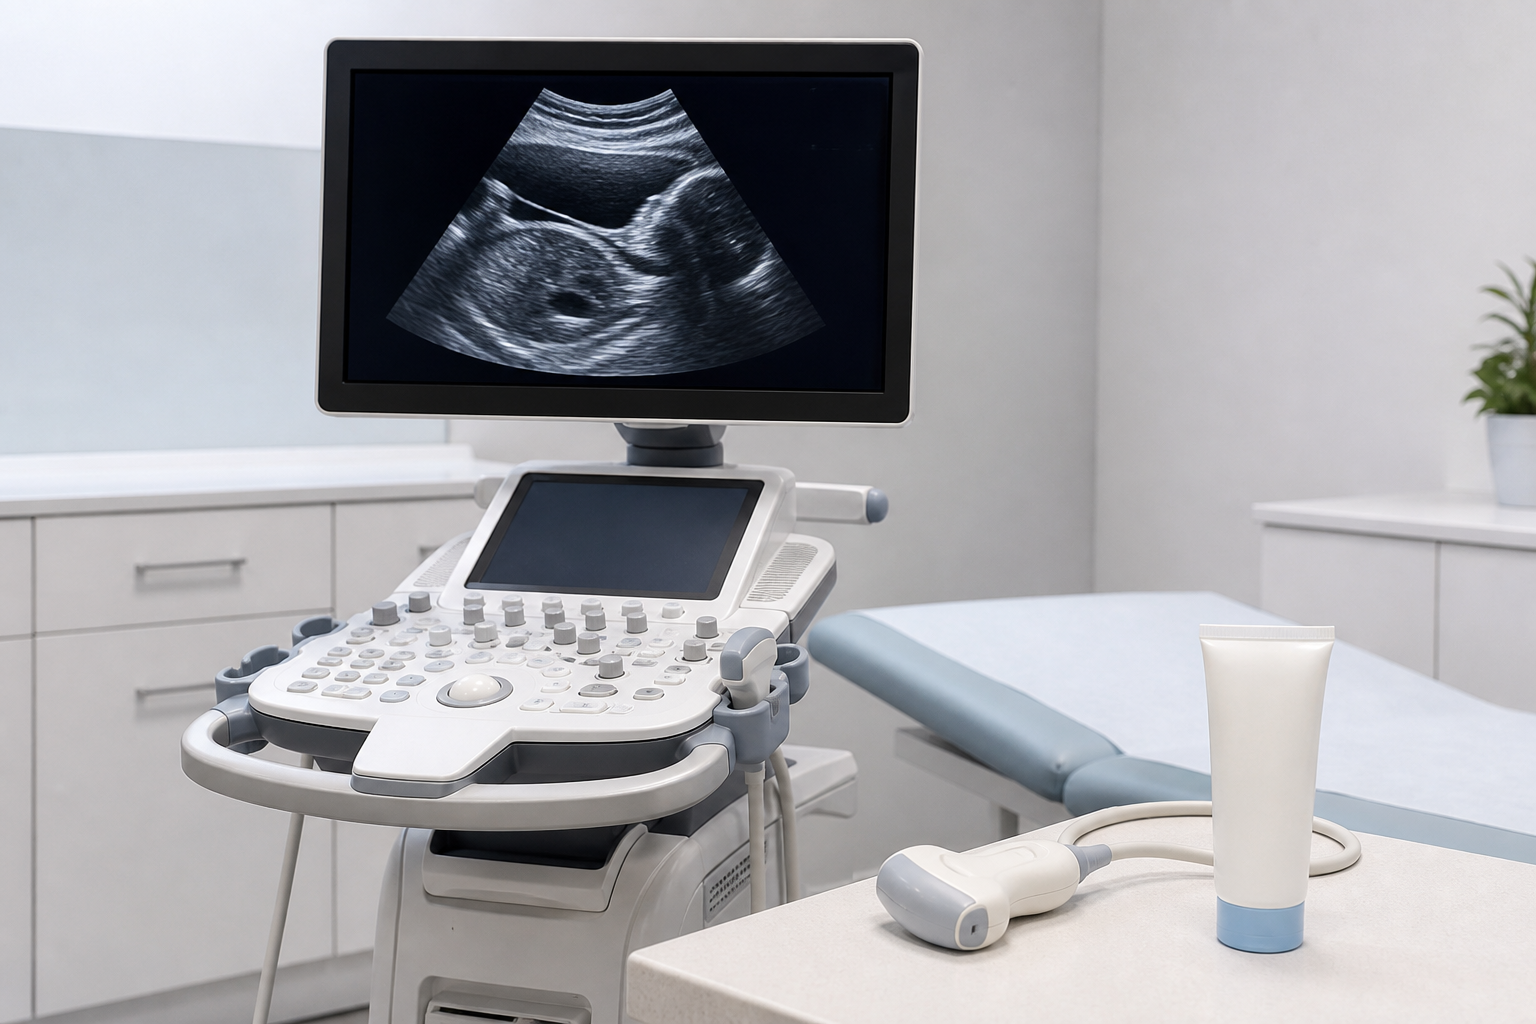
\includegraphics[width=0.58\linewidth]{images/book4/ai/b4-07-ultrasound-probe.png}

{\small Un ecógrafo: unos pocos megahercios de sonido, ecos cronometrados y los saltos de impedancia entre tejidos dibujan la imagen; el gel elimina la película de aire que lo reflejaría todo.}
\end{omfigure}

\section{Problema: del trueno al ecógrafo}

\begin{problem}[{Problema de fin de semana --- el sonido al aire libre, en
una sala de conciertos, dentro del cuerpo y en una sirena que pasa}]
\label{pb:b2:sound-waves:1}

Aire: $\gamma = 1.40$, $M = \qty{29}{g/mol}$, $Z = \qty{410}{kg.m^{-2}.s^{-1}}$ a
\qty{15}{\degreeCelsius}; $R = \qty{8.31}{J/(mol.K)}$.

\medskip
\noindent\textbf{Parte I --- La tormenta.}
\begin{enumerate}
  \item \omterm{thm:b2:sound-waves:equation}{Velocidad del sonido} a \qty{15}{\degreeCelsius} y a \qty{30}{\degreeCelsius};
        justifíquese la regla de ``tres segundos por kilómetro''.
  \item El trueno llega \qty{4.0}{s} después del relámpago: distancia del
        rayo. El trueno dura varios segundos aunque el relámpago sea
        instantáneo: ¿por qué?
  \item Cerca del rayo el nivel alcanza \qty{120}{dB}: amplitud de presión
        y amplitud de velocidad del aire.
  \item Energía recibida por metro cuadrado de pared durante un trueno de
        \qty{2}{s} a \qty{120}{dB}.
  \item En una noche despejada el suelo se enfría y el aire está más frío
        abajo que arriba. Los rayos sonoros obedecen la ley de Snell entre
        capas, $\sin i/c = $ const.: ¿se curvan hacia abajo o hacia arriba
        los rayos lanzados hacia arriba? ¿Por qué se oyen tan bien los
        sonidos lejanos de noche y sobre el agua?
  \item De día ocurre lo contrario: un oyente situado a \qty{3}{km} no oye
        nada. Estímese el ángulo que ha girado un rayo horizontal después
        de \qty{3}{km} si $c$ baja un \qty{1}{\%} por cada \qty{500}{m} de
        altitud (trátese la curvatura como uniforme: el rayo es un círculo).

  \item El aire absorbe las frecuencias altas mucho más que las bajas:
        ¿por qué retumba el trueno lejano y chasquea el rayo cercano?
\end{enumerate}

\medskip
\noindent\textbf{Parte II --- El concierto.}
Un altavoz recibe \qty{100}{W} de potencia eléctrica y convierte el $2\%$
en sonido, radiado por igual hacia el semiespacio que tiene delante.
\begin{enumerate}[resume]
  \item Potencia acústica; intensidad y nivel a \qty{10}{m}.
  \item Amplitud de presión allí; amplitudes de velocidad y de
        desplazamiento a \qty{100}{Hz}.
  \item Nivel a \qty{1}{m} (¿es seguro?) y distancia a la que la música
        baja a \qty{60}{dB}.
  \item Diez altavoces idénticos repartidos por el escenario y sin estar
        en fase: nivel a \qty{10}{m}. Dos altavoces alimentados en fase, a
        la misma distancia de un oyente situado sobre su eje: nivel allí.
  \item La sala (de volumen \qty{10000}{m^3}) tiene \qty{2000}{m^2} de paredes y público que absorben el $30\%$ del
        sonido que les llega: estímense la energía acústica almacenada en
        la sala en equilibrio y el tiempo de reverberación (el que tarda
        el nivel en bajar \qty{60}{dB} tras cesar la música), usando el
        balance entre la potencia emitida y la potencia absorbida
        ($I_{\text{pared}} \approx ce/4$ para un campo difuso, admitido).
\end{enumerate}

\medskip
\noindent\textbf{Parte III --- El ecógrafo.}
Tejido blando: $c = \qty{1540}{m/s}$, $Z = \qty{1.6e6}{kg.m^{-2}.s^{-1}}$; hueso
$Z = \qty{7e6}{kg.m^{-2}.s^{-1}}$; aire $\qty{400}{kg.m^{-2}.s^{-1}}$. Con incidencia
normal, la amplitud de presión reflejada en una interfaz vale $r = (Z_2 -
Z_1)/(Z_2 + Z_1)$ veces la incidente (deducido en
\cref{ch:b2:wave-interfaces}); el tejido atenúa el sonido unos
\qty{0.5}{dB} por centímetro y por megahercio.
\begin{enumerate}[resume]
  \item Longitud de onda en el tejido a \qty{3}{MHz}, \qty{5}{MHz} y
        \qty{10}{MHz}; el detalle más pequeño que cada una resuelve es de
        alrededor de una longitud de onda.
  \item Retardo del eco de un órgano situado a \qty{12}{cm} de
        profundidad; ritmo máximo al que pueden enviarse pulsos sin
        confundir ecos; tiempo para formar una imagen de $200$ líneas.
  \item Fracción de la presión, y de la energía, reflejada en una interfaz
        tejido--aire; en una tejido--hueso; y entre grasa
        ($Z = \qty{1.38e6}{kg.m^{-2}.s^{-1}}$) y músculo
        ($\qty{1.70e6}{kg.m^{-2}.s^{-1}}$). ¿Por qué el gel y por qué dan
        sombra los huesos?
  \item A \qty{5}{MHz} el haz atraviesa \qty{2}{cm} de grasa antes de
        encontrar músculo: fracción de la energía emitida que vuelve a la
        sonda desde esa interfaz (reflexión y atenuación de ida y vuelta),
        en \omterm{def:b2:sound-waves:decibel}{decibelios}.
  \item Atenuación de ida y vuelta en \omterm{def:b2:sound-waves:decibel}{decibelios} para el órgano de la
        pregunta 12 a cada una de las tres frecuencias; si el aparato
        admite \qty{80}{dB} de pérdida, ¿qué frecuencias sirven? Enúnciese
        el compromiso entre resolución y profundidad.
  \item La sonda emite pulsos de \qty{1}{\micro s} a \qty{5}{MHz}: ¿cuántas
        longitudes de onda dura un pulso y cómo limita eso la resolución
        en profundidad?
  \item Modo Doppler a \qty{5}{MHz} sobre una arteria a \qty{0.40}{m/s}, con
        el haz a \qty{60}{\degree}: desplazamiento; qué oye el operador.
\end{enumerate}

\medskip
\noindent\textbf{Parte IV --- La sirena.}
\begin{enumerate}[resume]
  \item Una ambulancia pasa a \qty{90}{km/h} con una sirena de \qty{700}{Hz}:
        frecuencias que se oyen al acercarse y al alejarse; intervalo
        entre ambas en semitonos (un semitono es una razón $2^{1/12}$).
  \item El oyente va en un coche a \qty{15}{m/s} hacia la ambulancia que
        se acerca: frecuencia que oye.
  \item ¿En qué instante oye exactamente \qty{700}{Hz} un oyente que está
        en la acera?
  \item Los frentes de onda de la ambulancia por delante de ella: longitud
        de onda; celeridad del sonido respecto de la ambulancia por delante
        y por detrás.
  \item Un cinemómetro de \qty{24}{GHz} mide un desplazamiento de
        \qty{3.2}{kHz} en un coche: celeridad del coche (la onda se
        desplaza dos veces).
  \item Resúmase: las seis celeridades de este problema (sonido en el
        aire, en el tejido, la ambulancia, el coche, los glóbulos rojos y
        la luz) y la única fórmula que las trata a todas.
\end{enumerate}
\end{problem}
